\chapter{User Documentation}

In this chapter we will explore the usage of the program from the perspective of and end user. We define the minimum requirements for the programs running, provide ways for installation and show example usages of the program.

\section{Program requirements}

The program can run on any 64 bit processor and is prepared to run on Windows and Linux operating system. The program can run with only a \ac{CPU} but for it to work with OpenGl it needs a \ac{GPU} that is capable to run atleast 1024 concurrent threads. The CUDA functionality requires an NVIDIA \ac{GPU} whit the same concurrent thread requirement.

\section{Installation guide}

The program requires no installation for an end user. You only need to download the provided compressed binaries for your operating system from the following website \href{https://github.com/Palnit/BSC-Thesis}{https://github.com/Palnit/BSC-Thesis} and unzip the binary and run. Currently there's 4 compiled binary: linux, linux-no-cuda, windows, windows-no-cuda. The no-cuda version binaries were created so the program can run on non CUDA compatible GPUs. If you want to build it for your self with CUDA capability you need to download the CUDA SDK from \href{https://developer.nvidia.com/cuda-toolkit}{https://developer.nvidia.com/cuda-toolkit} and CMAKE with a \CC\ build system e.g.: ninja, make and a compiler e.g.: \GG\ , MSVC, Clangd. There's two standalone programs one is for synthetic testing the other is for testing on real pictures. The synthetic tester's name is: BSC\_Thesis\_Tests, the real picture tester's name is: BSC\_Theis. 

\begin{figure}[H]
\begin{minipage}{.49\textwidth}
\begin{figure}[H]
\centering
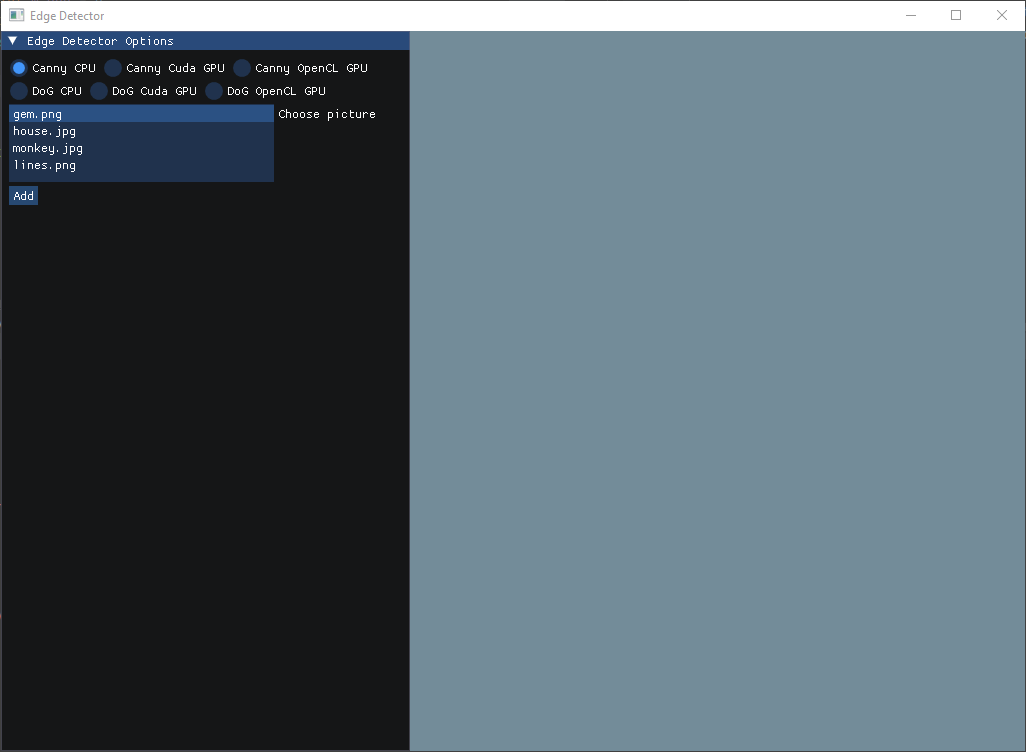
\includegraphics[width=\linewidth]{picture_window}
\caption{Program for real pictures}
\label{fig:noraml_prog}
\end{figure}
\end{minipage}
\begin{minipage}{.49\textwidth}
\begin{figure}[H]
\centering
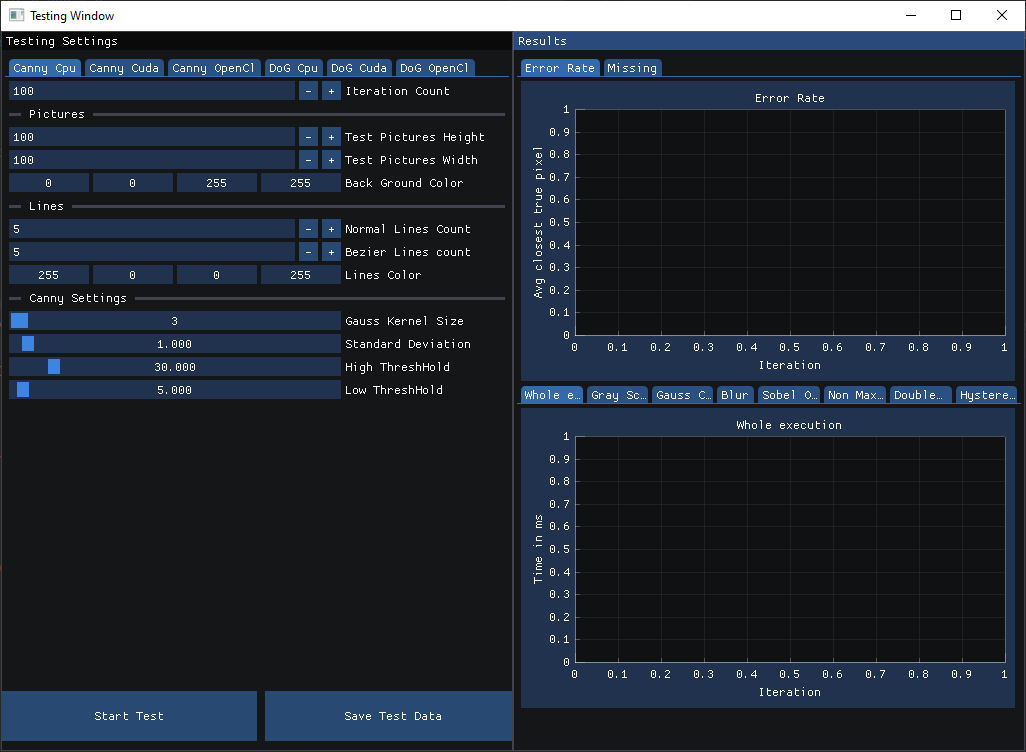
\includegraphics[width=\linewidth]{sintetic_tester}
\caption{Program for synthetic testing}
\label{fig:test_prog}
\end{figure}
\end{minipage}
\end{figure}

\section{Program Introduction}

In this section I will now demonstrate how the two programs work how to use them and what can what errors might occur during the usage of our program.

\subsection{Synthetic tester}
\label{chap:tester}

\begin{figure}[H]
\centering
\begin{minipage}[t]{.49\textwidth}
\centering
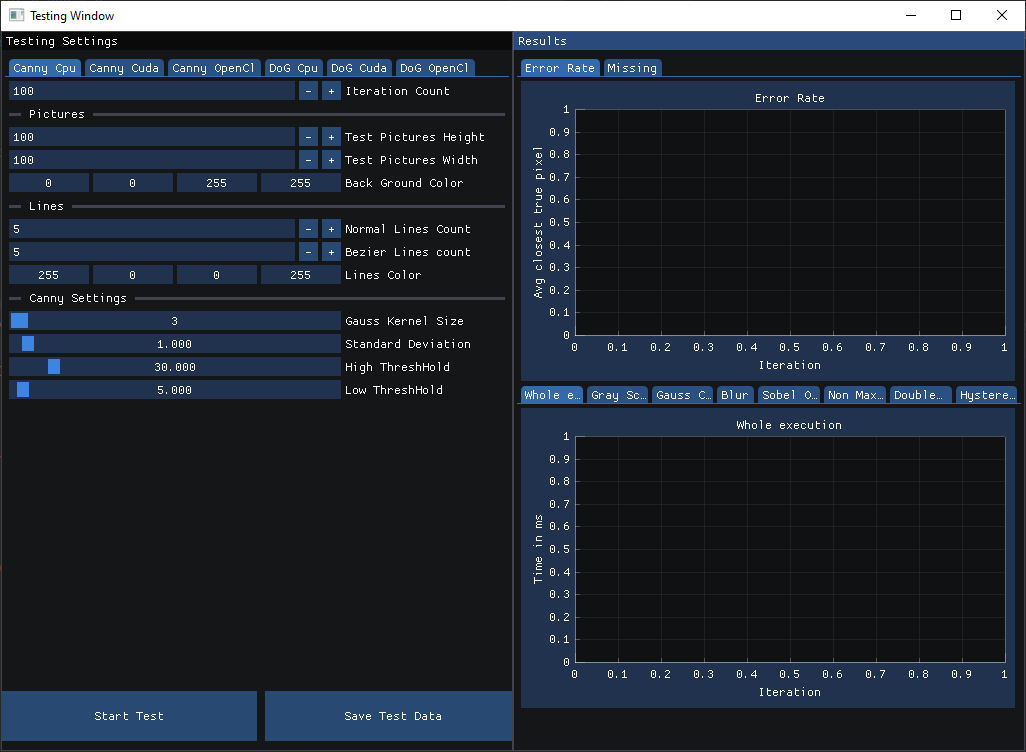
\includegraphics[width=\linewidth]{sintetic_tester}
\end{minipage}
\begin{minipage}[t]{.49\textwidth}
\centering
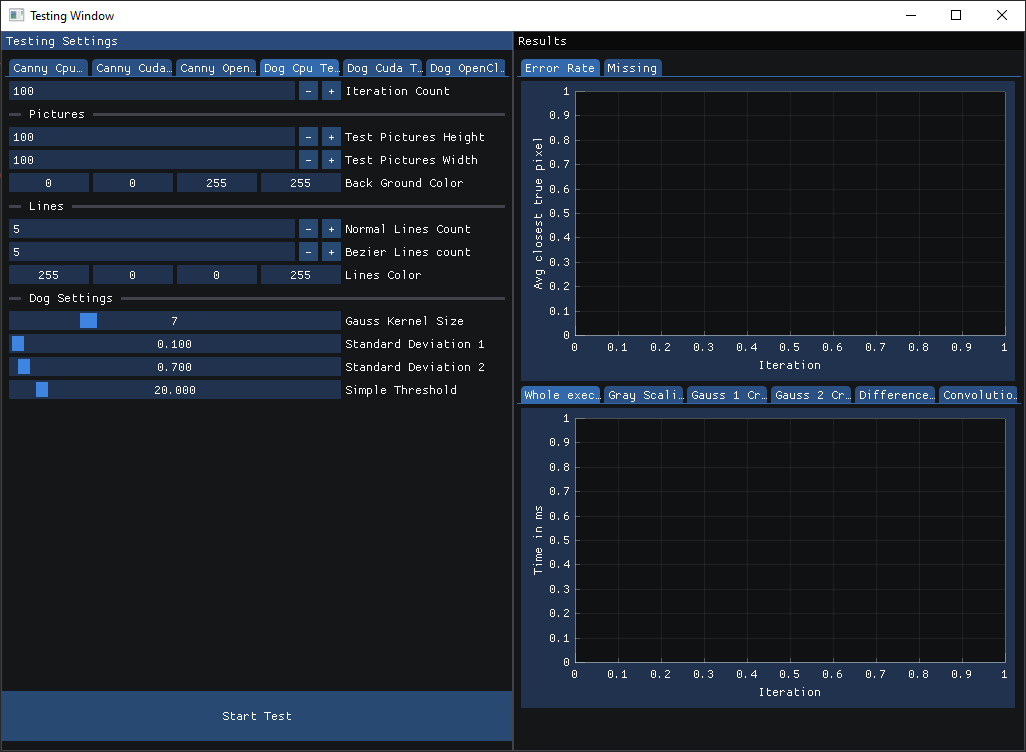
\includegraphics[width=\linewidth]{sintetic_tester_dog}
\end{minipage}
\caption{Difference between the settings of \ac{Canny} and \ac{DoG} detection pages}
\label{fig:test_prog_dem}
\end{figure}

For the synthetic tester see in \autoref{fig:test_prog_dem} in both pictures at the left side of the window are the settings for the tester. At the top I can choose which detector I want to test. Below that I can choose the test pictures settings I can set it's height, width, and base color. After that are the settings for the lines how many normal and curved lines I want and what color should they be. And lastly are the specific settings for the algorithm. 

If I choose to test the \ac{Canny} algorithm see in the left picture in \autoref{fig:test_prog_dem} there are 4 settings. The kernel size of the Gaussian blur, the standard deviation of sad kernel, and the high/low thresh holds of the \ac{Canny} algorithms this adjusts what pixel values should be kept these are kept low for the purpose to find the most pixels for the tests. 

As for the \ac{DoG} algorithm see in the right picture in \autoref{fig:test_prog_dem} there's 4 settings too. The first is the same kernel size as in \ac{Canny} algorithm this will set the size for bot kernels used in the algorithm. Below that there's to standard deviation for the two kernel's that will be used. And lastly there's a Simple threshold to be able to test accuracy, this is original not a part of the algorithm but we need it to be able to differentiate between detected pictures and undetected pictures because their values are not exact

This settings are needed to adjusts the algorithms to get the best results. Sadly we cannot write an algorithm that will find the edges that our human minds register and there can be many errors these settings are there to help make pictures clearer.

And lastly there's a button on the bottom of the page that will start the testing. The other button next to it is for saving the completed test data. If there were no tests no data will be saved. The original and the detected pictures are automatically saved this button only saves the timings, error rate and missing pixels count in a text file.

For the right side of the window it contains the test results data. At the top are the error rate and the missing pixel count. The error rate show for each iteration of the program how many pixels were detected that are not actual pixels. The missing pixels show how many of the original pixels from the lines were not detected in at all. Below these two are the graphs for the timings. Here we can take a look at how many \ac{ms} it took the program to finish each step of the algorithm. Lastly at the bottom of the right side are the averages of all the tests error rate and missing pixel count.

\subsection{Real picture tester}
\label{chap:real_pic_tester}

\begin{figure}[H]
\centering
\begin{minipage}[t]{.49\textwidth}
\centering
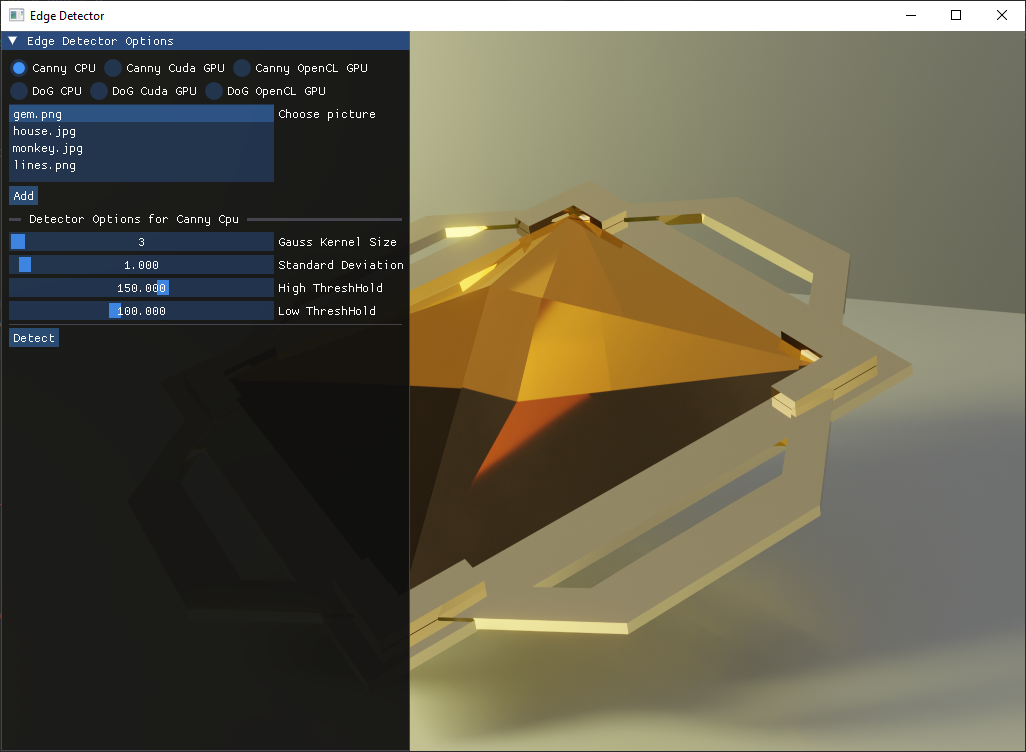
\includegraphics[width=\linewidth]{picture_window_pic}
\end{minipage}
\begin{minipage}[t]{.49\textwidth}
\centering
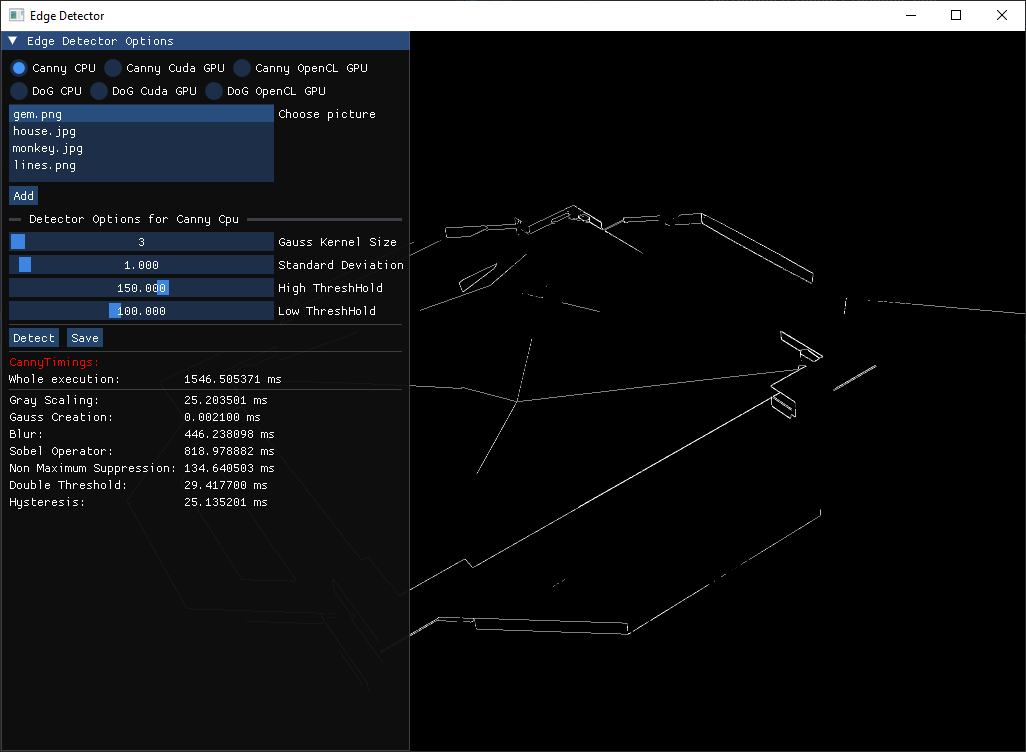
\includegraphics[width=\linewidth]{picture_window_detected}
\end{minipage}
\caption{The Difference of before detection after detection}
\label{fig:pic_prog_dif}
\end{figure}

For the real picture tester see in \autoref{fig:pic_prog_dif} this shows the actual actual pictures we are working on. This is because this doesn't operate on a large number of generated pictures and the reason for this programs existence is to show how the algorithm actually looks on a real picture.

Here there's only one window congaing the algorithm specific settings and the testers. At the top I have to choose which detector to use with what picture. Right now it only operates on pre defined pictures that's because this application is a tester to see what the results of the algorithms are. The program it self is ready to be used on any size of picture and any format of picture that the \ac{SDL2} library can load. This includes but not limited to the most popular: \ac{PNG} and \ac{JPEG}.

After choosing the detector is when the algorithm specific settings show up. These settings are the same that are in \autoref{chap:tester}. After choosing the settings for the algorithm pressing the detect button will start the algorithm and when it's finished the timings of the picture will be shown. There's no data for the missing pixels or how many erroneous detected pixels are since we cannot know that. I will go int details why in \autoref{chap:dev_testing}.